\chapter{Results}
\label{results}

\minitoc

In this chapter relevant articles gathered on ...

\newpage

\section{Introduction and Clarification}

\begin{table}[H]
\begin{center}
    \begin{tabular}{| p{5cm} | p{3.7cm} | p{1cm} | p{4cm} |}
    \hline
    \textbf{Article Name} & \textbf{Author(s)} & \textbf{Year} & \textbf{Keywords} \\ \hline
    Inter-team Coordination in Large-scale Globally Distributed Scrum: Do Scrum-of-Scrums Really Work? & Maria Paasivaara, Casper Lassenius, Ville T. Heikkilä & 2012 & Agile Software Development; Distributed Scrum; Global Software Engineering; Inter-team Coordination \\ \hline
    Communities of Practice in a Large Distributed Agile Software Development Organization – Case Ericsson & Maria Paasivaara, Casper Lassenius & 2014 & Communities of Practice; Large-scale Agile Software Development; Scaling Agile \\ \hline
    Operational Release Planning in Large-scale Scrum with Multiple Stakeholders – A Longitudinal Case Study at F-Secure Corporation & Ville T. Heikkilä, Maria Paasivaara, Kristian Rautiainen, Casper Lassenius, Towo Toivola, Janne Järvinen & 2015 & Agile Software Development; Scrum; Large Projects; Release Planning; Software Project Management \\ \hline
Towards a Governance Framework for Chains of Scrum Teams & Jan Vlietland, Hans van Vliet & 2015 & Agile; Chain of Scrum Teams; Coordination; Priority; Alignment; Predictability \\ \hline
    \end{tabular}
    \caption{Summary of articles used in this chapter.}
    \label{soauitc}
\end{center}
\end{table}

\begin{table}[H]
\begin{center}
    \begin{tabular}{| p{4cm} | p{8cm} |}
    \hline
    \textbf{Role} & \textbf{Description of role} \\ \hline
    Scrum master & \\ \hline
    Functional architect & \\ \hline
    Technical architect & \\ \hline
    Tester & \\ \hline
    Developer & \\ \hline
    \end{tabular}
    \caption{Team roles present in Scrum teams.}
    \label{trpist}
\end{center}
\end{table}

\begin{figure}[H]
\centering
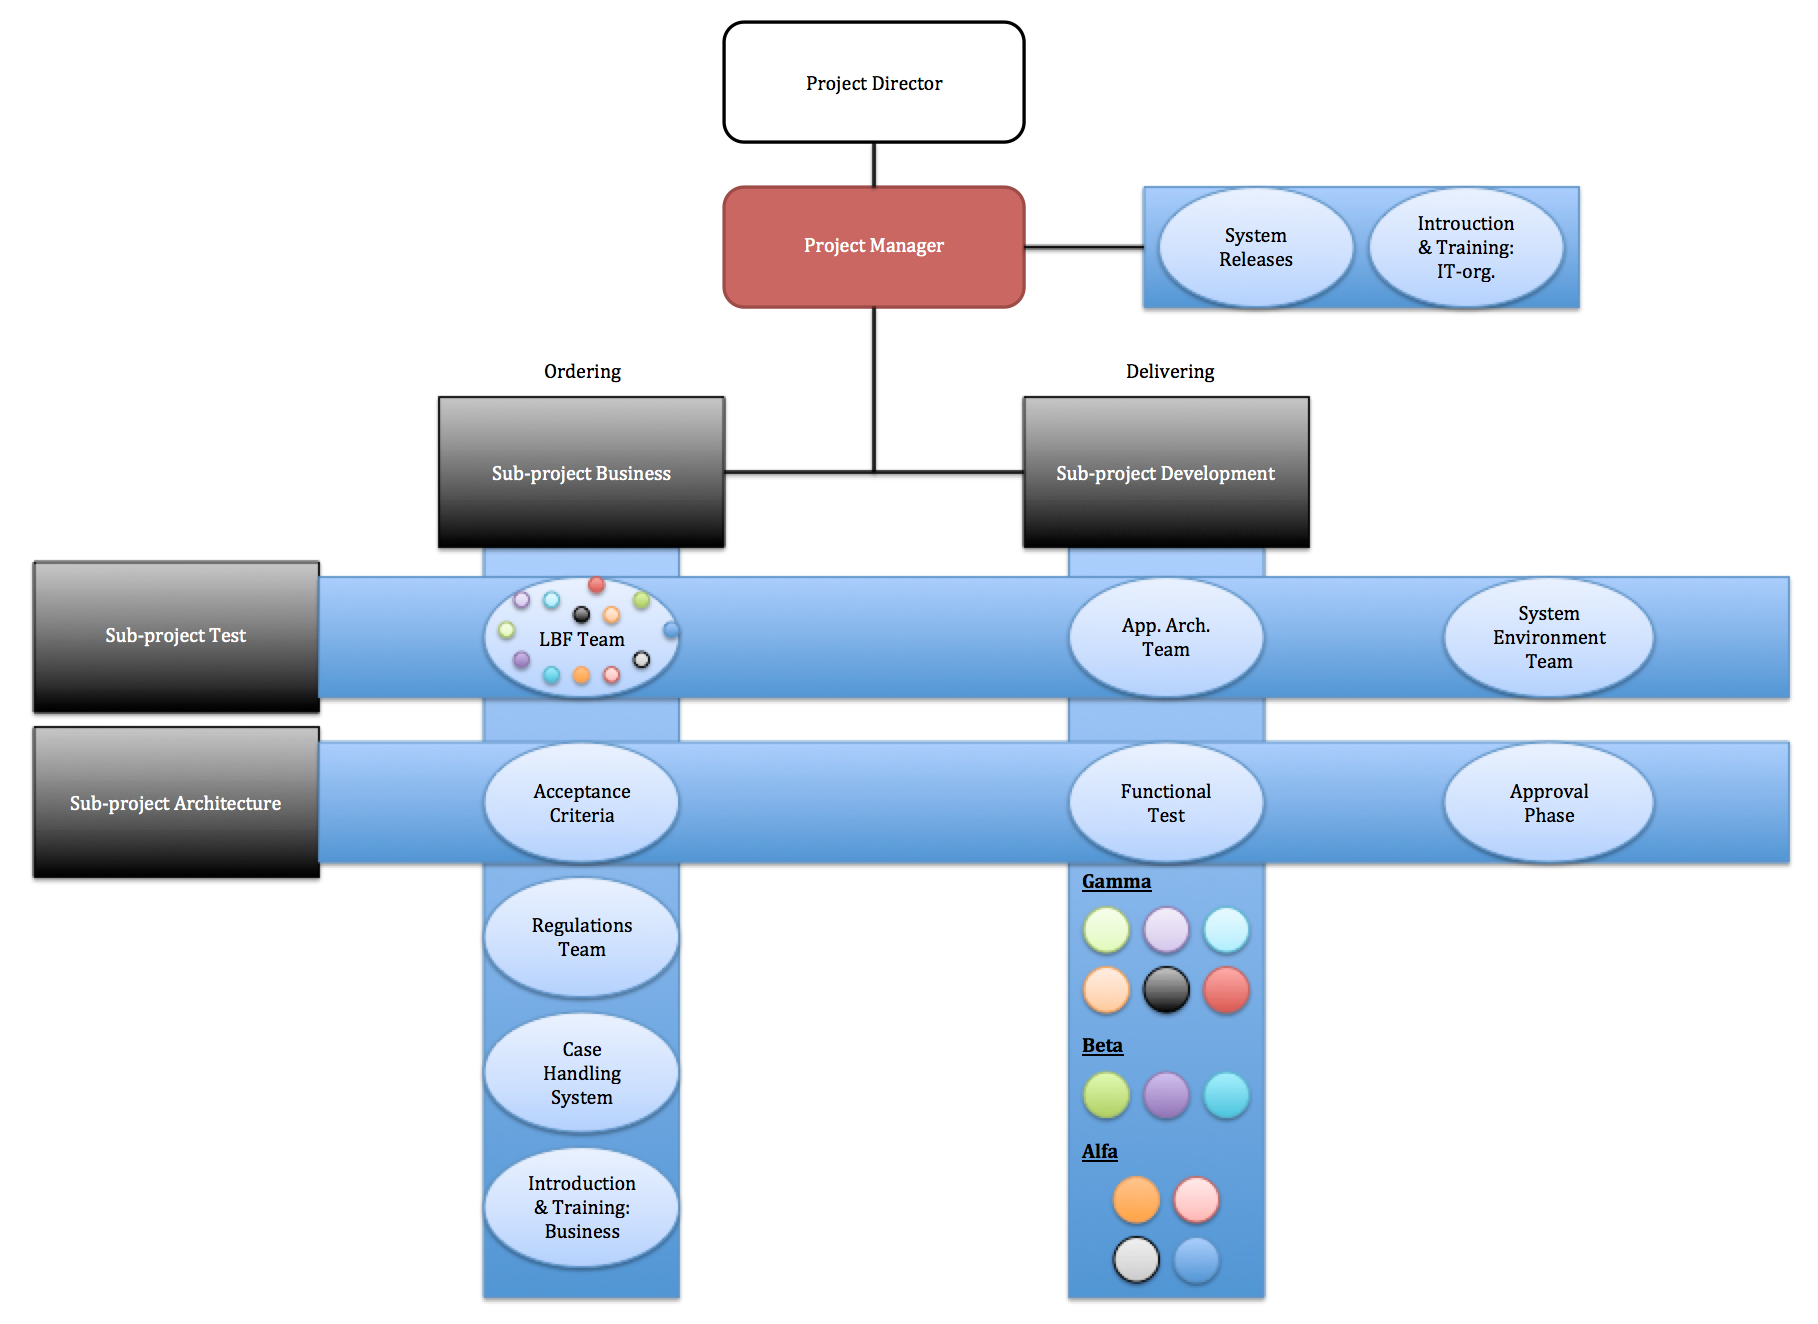
\includegraphics[trim = 40mm 0mm 7mm 0mm,width=180mm]{images/omega_organisation.png}
\caption{Omega-project's organisation.}
\label{omega}
\end{figure}

\begin{figure}[H]
\centering
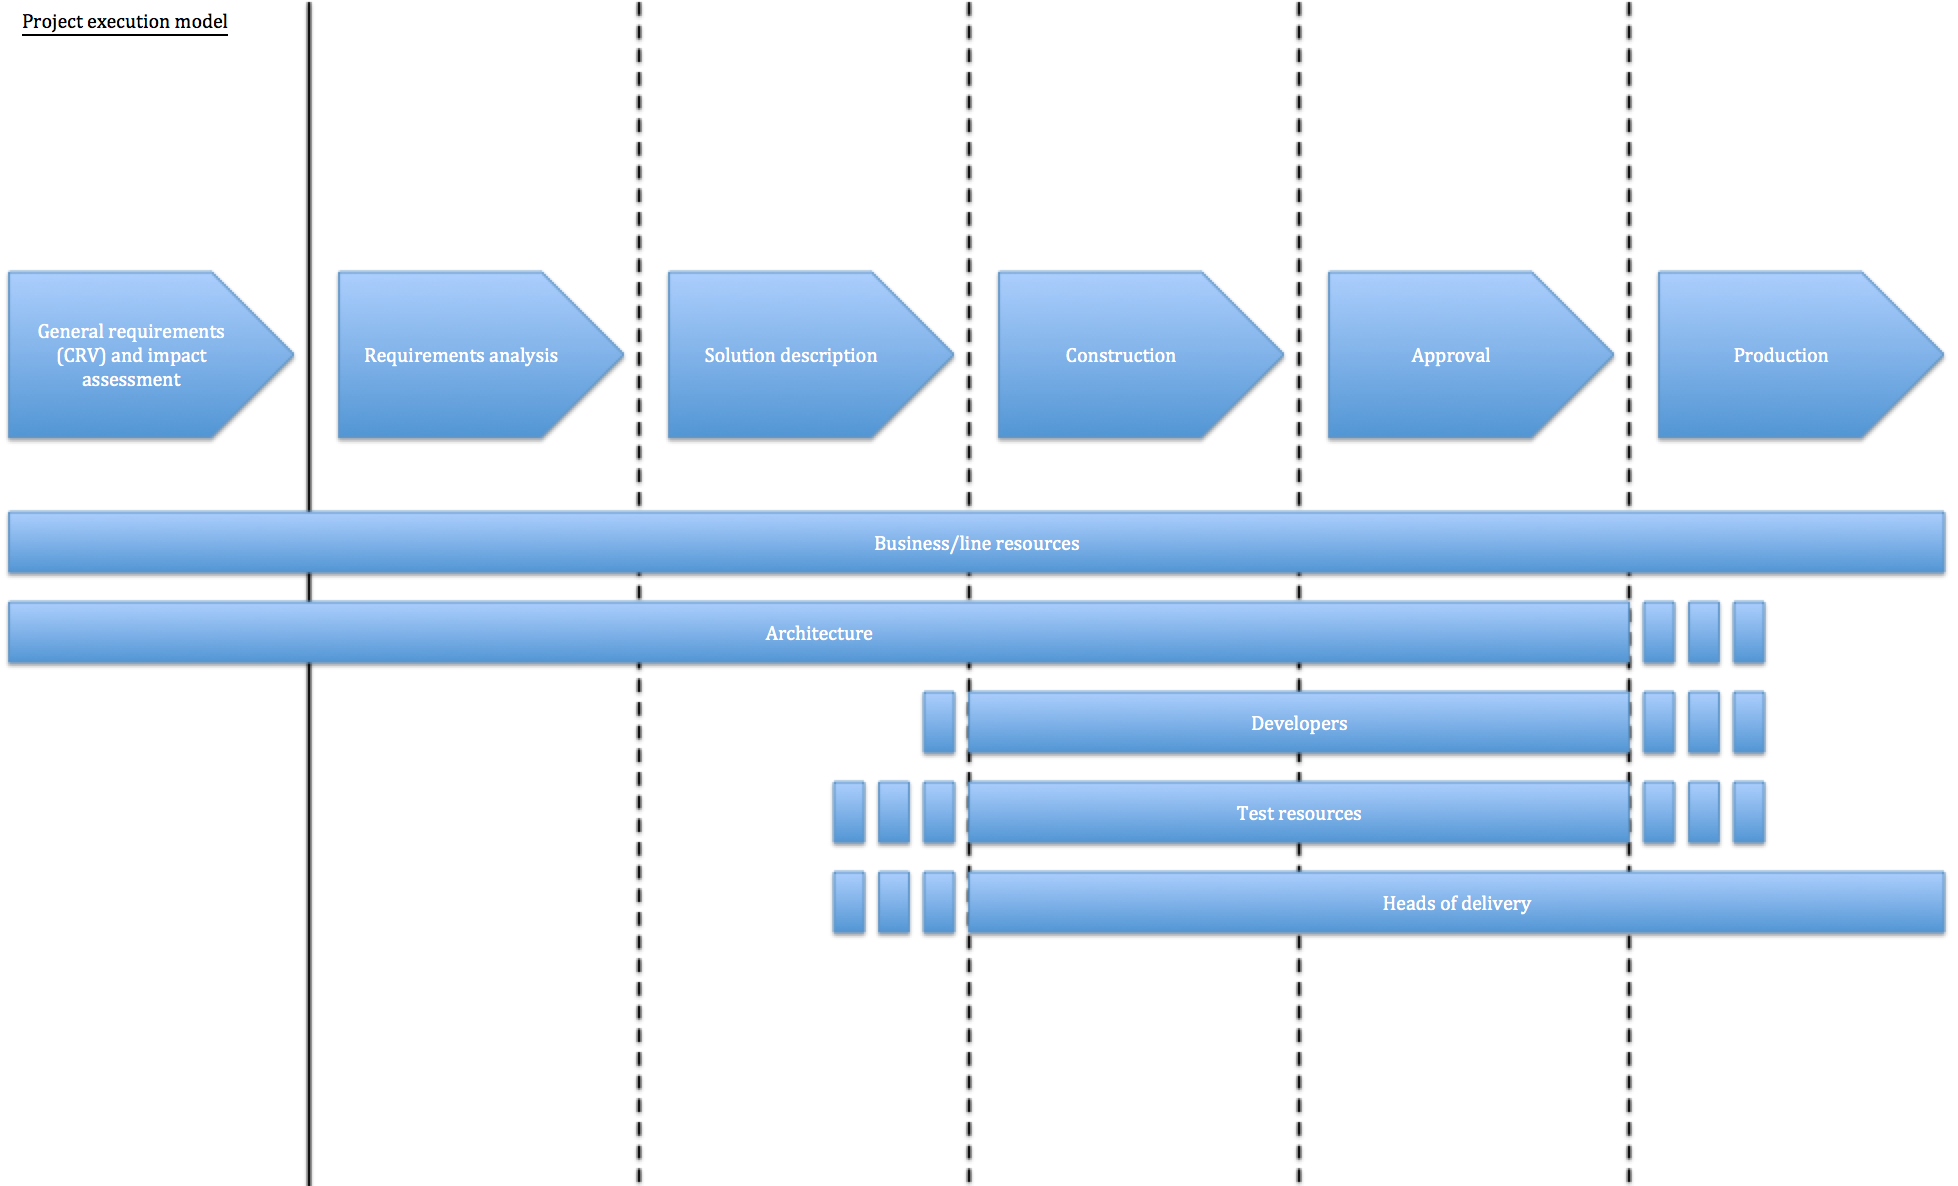
\includegraphics[angle=90, trim = 0mm 0mm 20mm 0mm,width=160mm, height=230mm]{images/execution_model.png}
\caption{Project execution model.}
\label{project_execution}
\end{figure}

\begin{figure}[H]
\centering
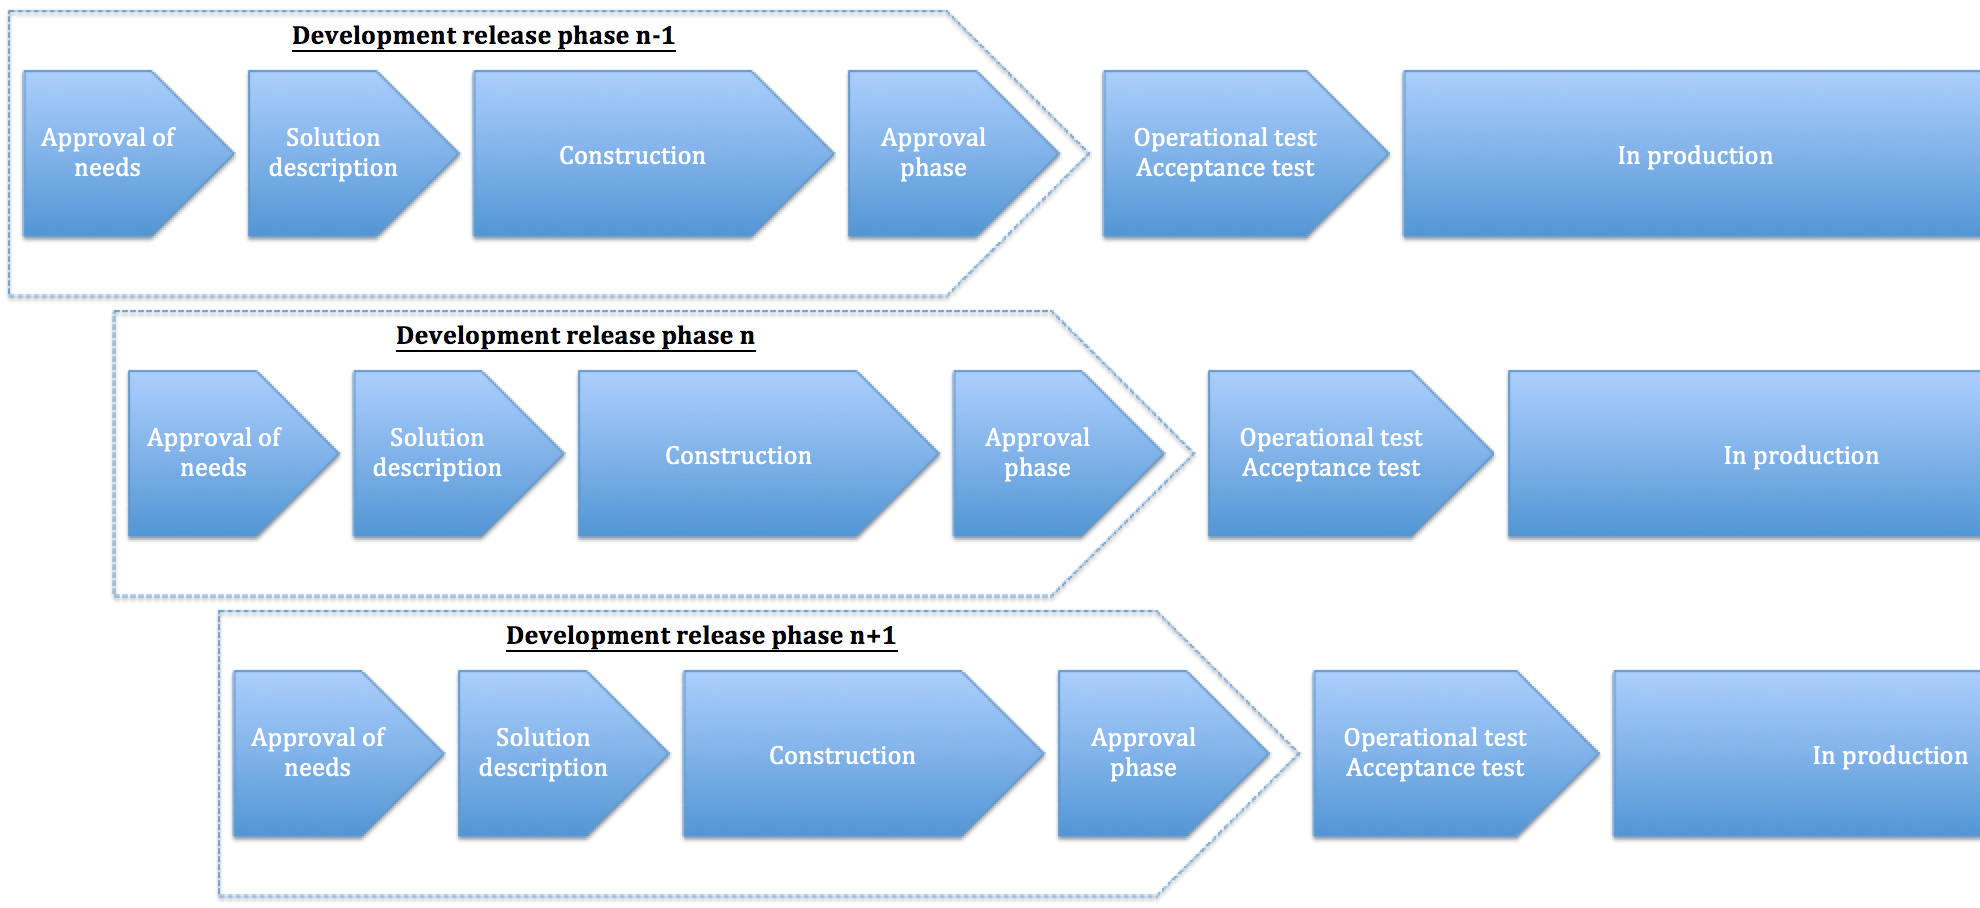
\includegraphics[angle=90, trim = 0mm 0mm 20mm 0mm,width=160mm, height=230mm]{images/initial_development_process}
\caption{Initial development process.}
\label{initial_development_process}
\end{figure}

%\begin{table}[H]
\begin{center}
    \begin{longtable}{| p{6cm} | p{9cm} |}

    \hline \textbf{Coordination mechanism} & \textbf{Description of mechanism} \\ \hline
    \endfirsthead

    \multicolumn{2}{c}%
{{\bfseries \tablename\ \thetable{} -- continued from previous page}} \\ \hline
    \textbf{Coordination mechanism} & \textbf{Description of mechanism} \\ \hline
    \endhead

    \multicolumn{2}{|r|}{{Continued on the next page\ldots}} \\ \hline
    \endfoot

   \endlastfoot

    Metascrum & A meeting similar to Scrum of Scrums but with less details which was held twice per week. Attending the metascrum was the project leaders and all the sub-project leaders from test, architecture, business and development. A ``technical metascrum'' was tried, but was shortly shut down after initiation. \\ \hline
    Planning day & The planning day was a form of kick-off for each sprint iteration where the project members met up with the project owner. The planning day was performed on three levels: project, organisation (Alpha, Beta and Gamma) and team. A rough sketch of the focus areas and work to be performed in the coming sprint was presented with a distribution towards each of the three organisations by the project owner. After this the organisations distributed the work on their respective teams, and lastly the teams got together separately and worked out a contract with estimated work to be performed which was delivered to the project owner team. Before the planning day commenced the developers also had a ``developer forum'' where development-oriented information and discussion was carried out. This was however held on an organisation basis, and not across the three organisations. \\ \hline
    Demo & Demo presentations were held by all Scrum teams at the end of each sprint iteration where everyone could attend. Each team was allocated approximately 10 minutes. There were also larger demo presentations for the project owner when a new release was finished. Some teams in addition started performing smaller demo sessions within the iterations to get rapid feedback. \\ \hline
    Pre-planning day & Before the ``planning day'' was carried out a pre-planning day was performed. Here typically different types of architects (especially functional architects) and the project owner (as well as some other members of the project owner's team) met to create a rough classification and allocation of work to the different Scrum teams for the coming sprint iteration. The allocated work was listed in a prioritised manner. \\ \hline
    Dependency meeting & A meeting held between all Scrum masters from the Alpha, Beta and Gamma teams. This meeting was held on the ``Planning day'' where the focus was on discovering dependencies across Scrum teams. However, these meetings faded away early on because of the dependencies being discovered and handled elsewhere. \\ \hline
    Solution description / ``Master plan'' & At the start of the Omega-project a larger solution description phase was performed involving a lot of architects (as can be seen from figure \ref{project_execution}). This lead to a ``master plan'' for the project and was documented in an issue tracker program called Jira. The ``master plan'' was continuously altered throughout the course of the development phase as outlined in figure \ref{initial_development_process}. In the solution description meetings important aspects were discussed such as coordination across organisations and management of activities. An example of what came out of these meetings was a dependency map of the whole Omega-project, which was in constant change. Part of the solution description meetings were also negotiation and estimation meetings which were important for the contract for each release. \\ \hline
    Jira and Wiki/Confluence & Different programs and forums were used for documentation and tracking within the project. In Jira all user stories and epics were located, and different information about the project and current sprint iteration could be seen on different levels, such as project and team level. The dependency map for the whole Omega-project was also located in Jira. Confluence was the main program used as a wiki. Here solution descriptions, team routines, routines across teams, system documentation, check lists, retrospectives, architectural guidelines, functional test etc. were all located. \\ \hline
    Open-space & An arena held on a voluntary and need basis, which was used for exchanging experiences. Only used during a few of the releases. Participants suggested the topics beforehand, leading to agendas for open-space sessions. \\ \hline
    Jabber & Jabber was introduced as an instant messaging service in the Omega-project after being identified as something needed in one of the Open-space sessions. Project members could ask both formal questions, e.g., technical questions, and informal questions or activities, e.g., wine lotteries. \\ \hline
    Lunch seminars & Kind of similar to the ``open-space'' sessions. Typically two to three topics were held by project-personnel on relevant and interesting topics, often regarding themes correlated to the current situation of the project. As with the ``open-space'' session these seminars were also held on a certain period of the project before fading away. \\ \hline
    Front-end meeting & The front-end developers worked with a complex framework called Flex. Because of this a lot of coordination had to be handled between teams working with this framework from all organisations. Therefore, front-end meetings where held were typically the most prominent Flex-developers were present. \\ \hline
    Technical architecture forum & At the technical architecture forum all technical architects met up to discuss what was to be done in the coding base to prevent coordination issues. These meetings were slowly fading away because the need was covered in other arenas. \\ \hline
    Architecture council & At these gatherings an architecture council listened to all team architects present their respective team's tasks for each sprint iteration. \\ \hline
    Business meeting & The business part of the Omega-project was coordinated through meetings where the business architects from Alpha, Beta and Gamma met up with the business unit from the project owner. Here the sprint iteration queue, and the current status of the project and sprint was presented. This meeting was held around one time each week or every other week. \\ \hline
    Bug-board discussion & The quality assurance unit with its testers had frequent meetings around bug-boards, especially after new releases and around acceptance testing. In the period after a new release these meetings were often held on a daily basis. Here all the bugs were gone through and allocated to the responsible Scrum team in either Alpha, Beta or Gamma. \\ \hline
    
    \caption{Coordination mechanisms used across the whole Omega-project.}
    \label{cmuatwo} 
    \end{longtable}
\end{center}
%\end{table}

\begin{center}
    \begin{longtable}{| p{6cm} | p{9cm} |}

    \hline \textbf{Coordination mechanism} & \textbf{Description of mechanism} \\ \hline
    \endfirsthead

    \multicolumn{2}{c}%
{{\bfseries \tablename\ \thetable{} -- continued from previous page}} \\ \hline
    \textbf{Coordination mechanism} & \textbf{Description of mechanism} \\ \hline
    \endhead

    \multicolumn{2}{|r|}{{Continued on the next page\ldots}} \\ \hline
    \endfoot

   \endlastfoot

    Scrum of Scrums (SoS) & Scrum of Scrums were meetings held by all organisations (Alpha, Beta and Gamma) ranging from two to three times per week. In these meetings all Scrum masters from the corresponding organisation, as well as project management (project leader, test leader, head technical architect, head functional architect, business leader and development leader). The main goal of the SoSs was to identify and handle obstacles. There were also held a few SoS meetings across organisations to handle potential changes to the contracts. \\ \hline
    Technical corner & The ``technical corner'' was a meeting Beta had in an early stage of the project. It was held on Fridays for about 1-1,5 hour. Here team architects presented important themes for the Beta-members. After a while it was shut down because of lack of interest and topics. \\ \hline
    Experience forum & The experience forum was an arena established in the Alpha-organisation for exchanging experiences. Here Scrum masters and the development manager met to discuss topics such as retrospectives, the planning day, and how work was performed by the Alpha-organisation's Scrum teams. It could be seen as a coaching-session with exchange of ideas and thoughts. \\ \hline
    Retrospective & Retrospectives were used on several levels in the project. All of the organisations used it on a pure Scrum team level, but some also used it on both the solution description personnel and in the project management team. The retrospectives for each Scrum team were held after the demo on Fridays. Here negative and positive information and aspects were brought forward and documented in Confluence. A few ``global retrospectives'' were also tested but swiftly faded away. \\ \hline
    Technical and functional architecture meetings & Both technical and functional architects had separate meetings within the different organisations. These meetings were typically short and held on a weekly or biweekly basis. The meetings were as mentioned brief and were primarily used for status updates, and keeping the technical and functional managers up-to-date to make the cross-coordination meetings with the other organisations easier and more precise. \\ \hline
    Supplier meeting & At Alpha a supplier meeting was held by the project leader for all Alpha-members. The project leader contributed with practical information regarding the project. In these meetings different members held presentation on different topics such as clean code, test driven development and project guidelines to keep the technical level up to scratch on the personnel. \\ \hline
    Meeting about queue & Alpha also had a meeting regarding ``what was next in the queue?'', ``what is the next delivery?'', ``what is the status on current user stories?'' and ``what is it that we feel is needed to drive the queue forward?''. In these meetings was held with the functional architect, development manager and product owner from Gamma. \\ \hline

    \caption{Coordination mechanisms used across teams within the specific organisations (Alpha, Beta and Gamma) in the Omega-project.}
    \label{cmuasito}
    \end{longtable}
\end{center}

\begin{center}
    \begin{longtable}{| p{6cm} | p{9cm} |}
   
    \hline \textbf{Mechanism/Aspect} & \textbf{Description} \\ \hline
    \endfirsthead

    \multicolumn{2}{c}%
{{\bfseries \tablename\ \thetable{} -- continued from previous page}} \\ \hline
    \textbf{Coordination mechanism} & \textbf{Description of mechanism} \\ \hline
    \endhead

    \multicolumn{2}{|r|}{{Continued on the next page\ldots}} \\ \hline
    \endfoot

   \endlastfoot 

    Stand-up & Daily stand-ups were used on all Scrum teams in the project. Here obstacles, progression and possible needs were voiced around the Scrum-boards. Introduced by Gamma was also the way of organising the stand-up meeting such that they were held on different timeslots. This made it possible for members to attend several stand-ups if necessary. \\ \hline
    Board discussion & An important aspect for coordination, discussion and status updates in the project was the frequent use of whiteboards. The stand-up meetings were for instance held around these boards, and on these boards the workload for each sprint iteration was put up and updated as the sprint moved along. The backside of the boards were left open to carry out informal discussion when needed. \\ \hline
    Co-location & One of the biggest impacts on the project, and coordination, collaboration and communication within the project was the radical co-location. This co-location came at any early stage (with the introduction of Alpha and Beta in Omega) in the project where all teams, as well as project management, were located in an open-plan office space at the same floor. \\ \hline
    Project management in same location & In both Alpha and Beta management by ``walking around, talking around'' was brought up. Because the project management was located in the same office space as the other project teams it was easy for them to keep track and manage by just being present. With management being close by it was, e.g., possible for development managers to have informal communication with each Scrum master every day, making sure they were up-to-date on the progress. This lead to easier decision making and problem handling for the project management team. Another important and positive factor was that decision making could be taken rapidly through more informal arenas, as teams could address project management at once without having to book formal meetings every time a decision had to be made. \\ \hline
    Informal communication & Another important impact on the coordination and general information sharing was the extensive use of informal communication. These communication arenas seemed to be very important in the agile mindset because of the pressure on delivering within a short period of time. With the use of informal communication arenas decisions could be made faster than using formal arenas such as having to book meetings where, e.g., timeslots had to match for participants. As the project progressed the informal communication arenas were more and more present, often replacing some of the formal communication arenas. \\ \hline
    Joint coffee break & An informal communication arena that was present throughout the Omega-project was the ongoing discussion around the coffee machine area. There were even joint coffee breaks at 2PM every day. These informal meetings saw a growth as the project moved along. \\ \hline
    Pair-programming & Pair-programming was introduced by Beta and adopted by some of the other organisations. Often the pairs constituted of one senior and one junior developer. The main reasons for using pair-programming was to achieve a higher standard on the coding, increase knowledge (especially of junior developers) and to build better relationships and trust within teams. Pair-programming was also tested across teams, but was not deemed successful. \\ \hline
    Trust & Another important aspect of the project was trust, both within and across organisations, but also between the organisations (Alpha, Beta and Gamma) and the product owner. Trust was increased through several ways, e.g., social gatherings, co-location and a general openness culture. With the increase in trust between the different project-members there was an increase in informal communication arenas, and a decrease in formal ones, leading to more rapid decision making, in line with the agile mindset. \\ \hline
    Rotation of team members & At Beta some rotation of members across the Scrum teams happened. This was mainly to spread competence and knowledge across teams to make them more ``all round teams'' able to handle different types of work. There were also a few rotations because of personal chemistry. \\ \hline
    Rotation of team placement & Another decision made by Beta and Gamma was to change location within the office space of some teams. This was a deliberate move by the project management to achieve better collaboration and communication, especially on the informal level, between teams working on similar parts of the project. \\ \hline
    Alpha/Beta-personnel placed in Gamma teams & An aspect that might have been important both for trust and the informal communication was that both Alpha and Beta members were located in Gamma teams. This probably made it easier to get informal communication going at an early stage of the Omega-project because some members knew each other across the organisations already. \\ \hline
    Continuous planning and change & Self-organising was present at different levels in Omega such as team, organisation and project level. At the team level the teams changed their ways as the project moved along introducing new and removing old aspects, e.g., moving from pair-programming to individual programming when knowledge increased. At both the organisational level and the project level different communication arenas were changed on a need-basis. This had mainly to do with the respective arenas being covered elsewhere, e.g., through informal communication. Another part of the project where continuous planning and change was present was within the dependency mapping and solution description. \\ \hline
    3-level hierarchy from product owner & Mentioned by Gamma was the way the product owner was organised within the project. At the top of the food change the main product owner sat, then three representatives from the product owner were located at Alpha, Beta and Gamma, and at the bottom of the hierarchy the product owner had functional experts and architects inside or close to the teams. This led to easier decision making as the representatives further down the hierarchy could answer on the behalf of the product owner, or at least knew who to ask for the answer increasing the pace of development and problem solving. \\ \hline

    \caption{Other coordination mechanisms and important aspects.}
    \label{ocmaia}
    \end{longtable}
\end{center}